%!TEX root = ../main.tex

\chapter{Parameter Sweeps}

It is often of interest to explore the parameter space of a model. We may want to find what the value of some parameters should be, or maybe we want to find regions in parameter space where the model exhibits interesting behavior.

StochSS supports sweeps over one or two parameters. To set up a parameter sweep, simply click \textbf{Parameter Sweep}. Select the model that you want to analyze, the parameters you want to analyze, the upper and lower bound of the parameters, and the number of steps in each parameter.

First import the \emph{lotkavolterra\_concentration\_oscil} model from the \emph{Public Library}. Select this model in the parameter sweep main window, and run a two-parameter sweep over $k1$ and $k2$. Click \textbf{Run Local}, and wait for the computation to finish. Once it has finished, the output can be visualized on the \textbf{Job Summary} page, see Figure \ref{psweep-fig1}. You have to select a \emph{mapper} and a \emph{reducer}, and can view the average concentrations, the max- and min-values, as well as the variance. As an example, if the \emph{mapper} is `final time', and the reducer is `average', then that means that you will plot the average of the populations at the final time point. Another example is that the mapper is `average' and the `reducer' is `max'. That means that we first take the average of each trajectory, and then the maximum of each average. The final output is then visualized in a graph or heatmap.
\begin{figure}[!ht]
\centering
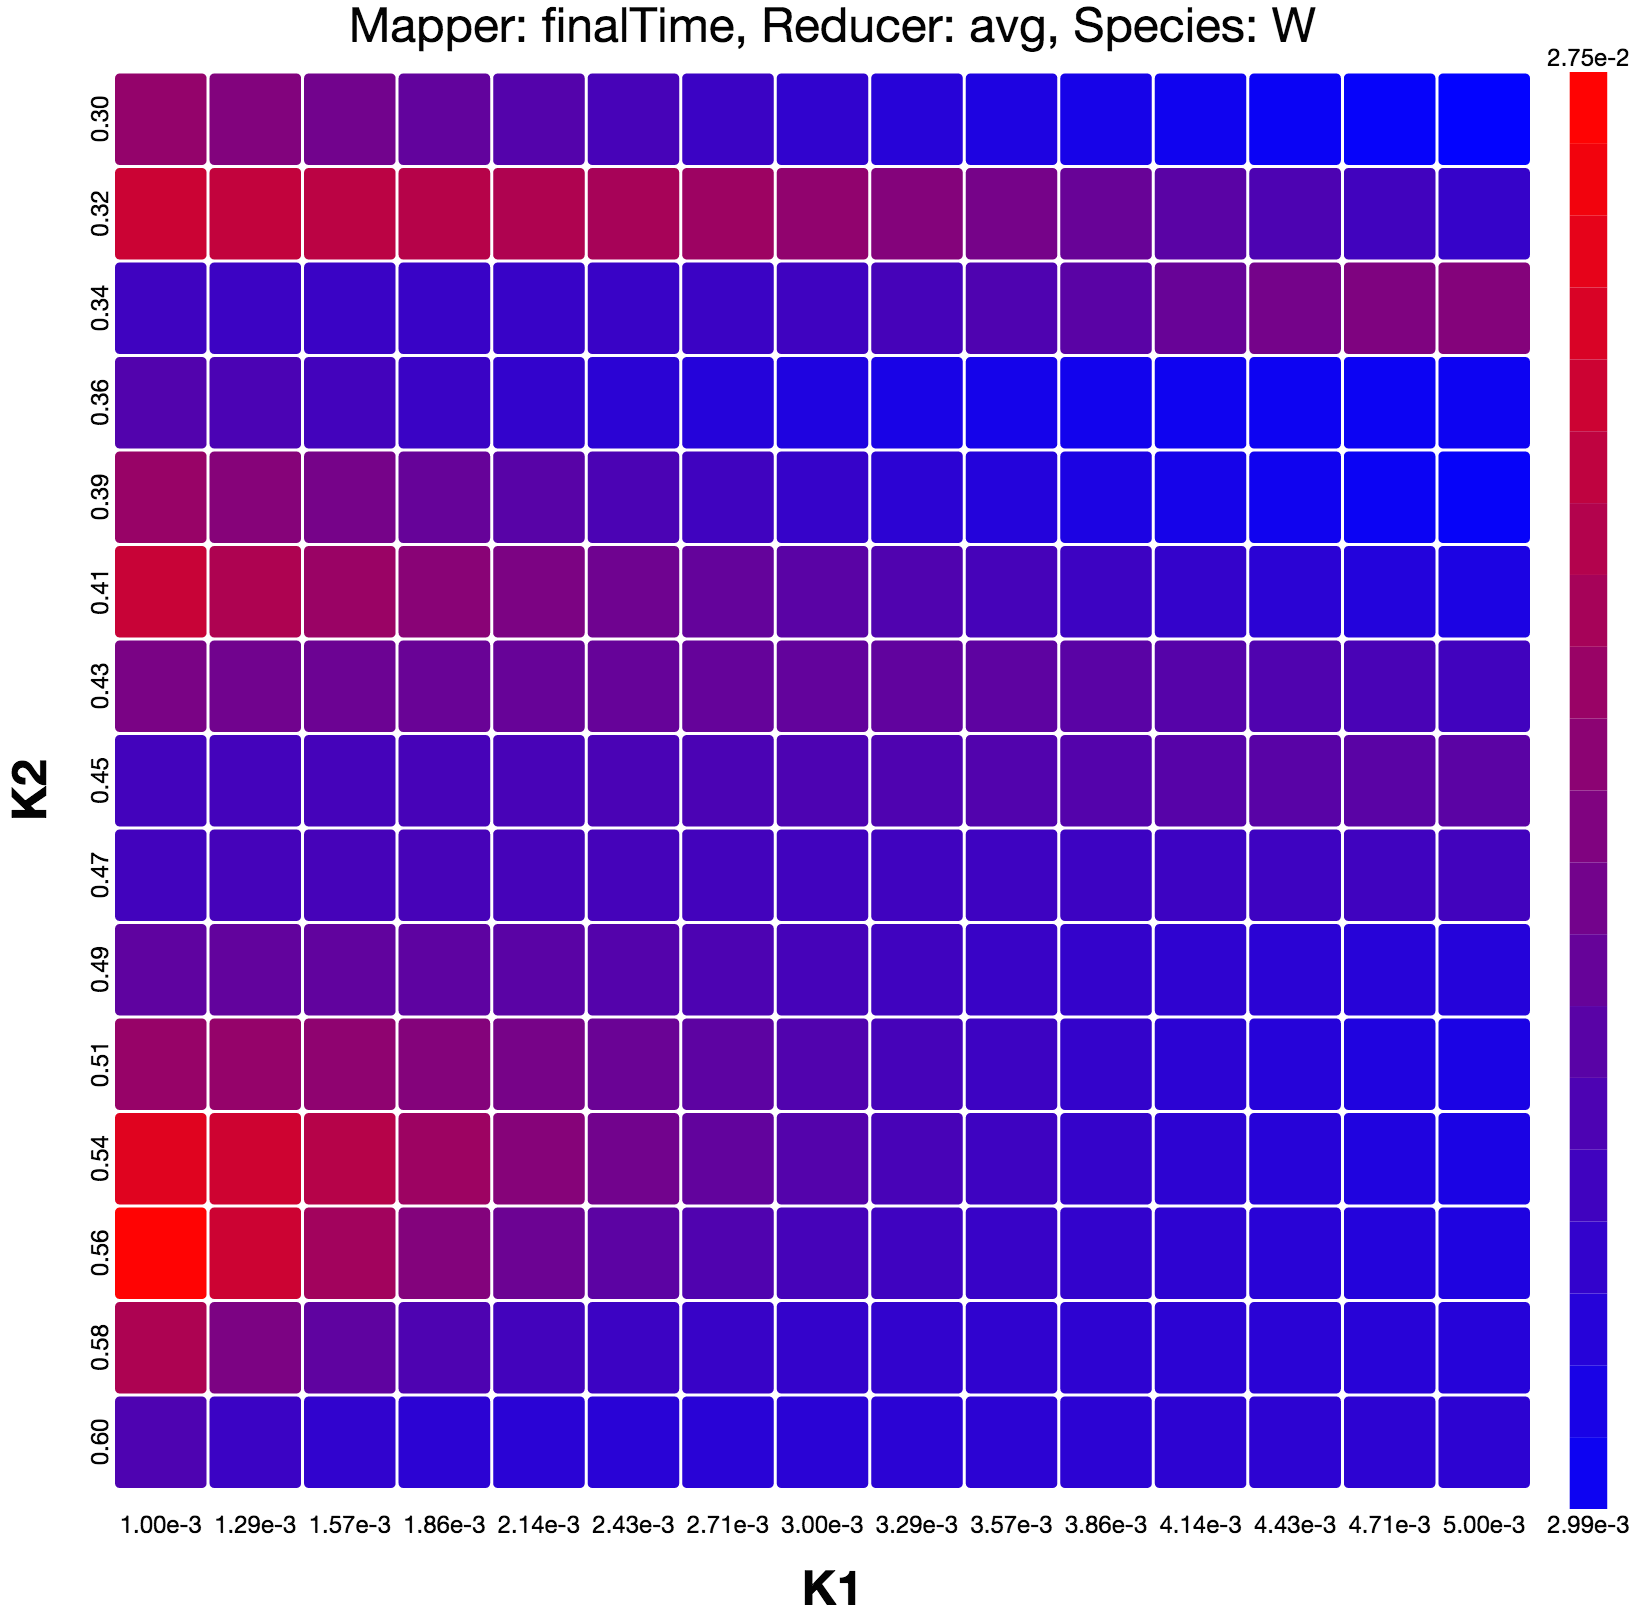
\includegraphics[width=0.95\textwidth]{Psweep/heatmap.png}
\caption{\label{psweep-fig1}A two-parameter sweep is visualized as a heat map. We have performed a sweep over the two parameters $k1$ and $k2$ of the \emph{lotkavolterra\_concentration\_oscil} model. The \emph{mapper} performs the initial analysis on the output---in this case simply taking the value of each solution at the final time point. The \emph{reducer} performs some analysis on the output of the mapper---in this case taking the average of the final time points. Note that this model is deterministic, and the average simply is the value of the ODE solution at the final time point.}
\end{figure}

Finally, if you need to perform an in-depth analysis of the data, there is the option of exporting the parameter sweep to a Jupyter Notebook. On the \textbf{Job Summary} page, click \textbf{Analyze using interactive Jupyter Notebook}. This launches a Jupyter Notebook, with a template for analyzing the data. We recommend users unfamiliar with Jupyter to visit http://jupyter.org for full documentation and tutorials. In short, it is an environment for interactive computing, and users can analyze and plot their data with Python scripts. For example, given a two-parameter sweep, we may ask ourselves which parameter values give a specific output value. While it is possible to estimate that by simply looking at the heatmap, that is likely unsatisfactory in a real modeling project. With the full scripting capabilities of Python, the user could automate and make this process rigorous by modifying the Notebook correspondingly.

